\chapter{Background and related work}\label{chap:related}

In this section, I will first give some brief introduction to the related research about software update in WSNs, and then I will describe some background research that is related to the major components of my proposed framework.

%\section{Control Logic}

\section{Software update in WSNs}

The existing WSN software update designs can be categorized according to {\em what} is to be transmitted over the network. 

The simplest solution is to transmit the complete new binary image to replace the old one on the sensors, e.g., Deluge (the default code distribution scheme in TinyOS~\cite{tinyos}).
The proposed schemes in this category mainly focus on how to package the new binary image and route the packets to the sensors under WSN constraints.
However, since the new binary and old binary share some common code segments, transmitting the complete image is not necessary and is a waste of energy.

Another approach is the {\em diff}-based design, which compares the code of successive versions and generates an edit script that summarizes the differences.
Only the script is transmitted to the remote sensors where the new code is re-generated by combining the old image and the edit script.  Since
less data is transmitted over the network, and the edit script is usually simple and can be easily interpreted by the sensors, the {\em diff}-based approach significantly improves energy-efficiency and has
become more popular in WSNs~\cite{related:script,stream,related:jeong-script,related:dynamic1,related:dynamic2,related:flexcup}.
The major focus of this category is how to compare the two binary versions and generate a small edit script.
However, because the code differences are derived from binaries generated using the {\em conventional compiler's code generation methods}, with possibly some optimizations, a simple change in the source code may result in many changes in the final binary. This has limited the {\em diff-}based approaches to only small updates such as fixing a ``bug''~\cite{related:script}.


The third approach transmits the binary code at different levels.  Some recent work introduced a small virtual machine~\cite{mate} or a dynamic linker~\cite{related:dynamic2,related:dynamic1} on the remote sensors. Instead of binary instructions, the code is represented at a higher level, e.g., virtual machine primitives,
which can minimize the code difference in many cases. The tradeoff is that these approaches introduce high runtime overhead and may consume more energy in the long run.


\section{Compiler}

Compiler is a program that can read a program in one language -- the \textit{source} language -- and translate it into an equivalent program in another language -- the \textit{target} language.~\cite{compiler}
The work flow of a compiler is shown as Figure~\ref{fig:compiler}.

\begin{figure}[htbp]
	\centering
		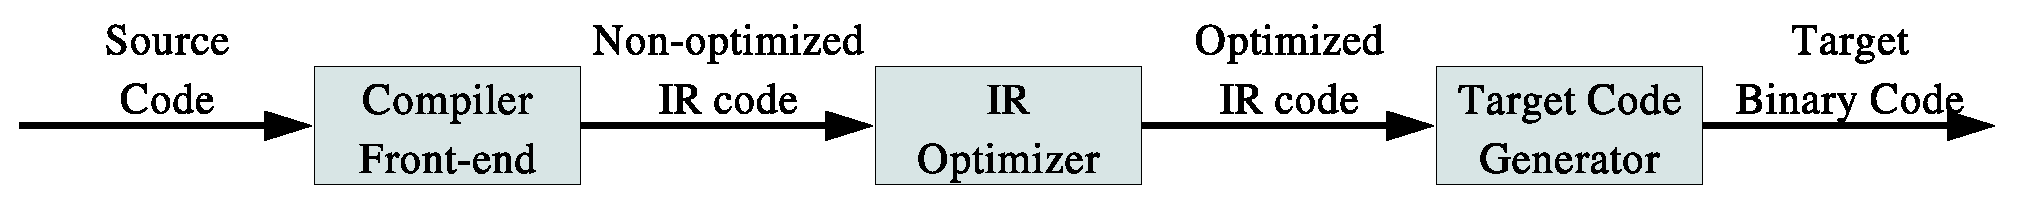
\includegraphics[scale=0.45]{figures/compiler.eps}
	\label{fig:compiler}
	\caption{Compiler work flow}
\end{figure}

The \textit{front-end} analyzes the source code to build an internal representation of the program, called the \textit{intermediate representation} or \textit{IR}. The \textit{IR} then is transformed into functionally equivalent but faster (or smaller) forms in the \textit{optimizer}. At the last stage, \textit{code generation}, the \textit{optimized IR code} is transformed into the target machine binary.

My study~\cite{ucc} has shown a small local source code change might cause a big difference in the binary. This is because if the source code level difference is minor and local, when translating such source code into IR code, the difference will also be localized, assuming a one-one mapping can be created between the source code and IR code. However, transforming the IR code to the target binary code may propagate such local differences into global differences, by applying data allocation, code placement, register allocation, etc. Thus, my update-conscious compilation design will focus on the code generation pass. The goal is to let the compiler preserve the semantic meaning of the source program while generating a similar code image with a given code image. Two key problems in code generation, register allocation and data allocation are studied in this research.

\subsection{Register allocation}

Registers are the fastest computational unit on the target machine, however, usually there are less registers than the values that need to be held. The goal of register allocation is to determine what values should be held by what registers. Because the values that are not held in registers reside in memory, and memory access takes longer time compared to register access, the efficiency of register allocation algorithm affects the execution efficiency of the program. 
Finding an optimal assignment of registers to variables is mathematically NP-complete. However, in the past twenty years, the register allocation problem has been extensively studied with great success in many aspects. 

\textbf{Traditional register allocation schemes} Graph coloring algorithms construct the variable interference graph and solve the global register allocation as a graph coloring problem~\cite{related:graph-color,related:graph-color-improvements,related:graph-color-iterated,related:graph-color-priority}. To achieve fast compilation, linear-scan algorithms assign variables to available registers through a simple scan of the program, instead of constructing the interference graph~\cite{related:linear-scan,related:linear-scan-fast}. It was reported that linear-scan allocators generate similar performance level code as those from graph coloring-based allocators, with a shorter compilation time required. Recently, the optimal or near optimal register allocation was formulated and solved through integer linear programming~\cite{related:ilp,related:ilp-cisc,related:ilp-fast} or multi-commodity network flows~\cite{related:ilp-progressive}.

However, all these register allocation algorithms listed above, target at generating code with better performance, in terms of less register spills. In the WSN software update management concept, we want to design an update-conscious compilation technique in order to reduce the size of update between different versions of one program or two programs that share common components. So these traditional register allocation schemes do not fit in our requirement.

\textbf{Update oriented register allocation}
Bivens and Soffa proposed the Incremental Register Allocation (IRA) scheme~\cite{related:ira} based on traditional graph coloring algorithm. While the software is update incrementally based on a previous version, the scheme only reallocates registers for the changed code, but preserves the assignment for unchanged code. 

Though it is designed for incremental compilation, its goal is to save compilation time, when minor software update occurs. It may generate similar register allocation results as the previous version unintentionally, yet it always follows the original register allocation for the unchanged code, which may lose the code performance when the source code update is relatively large. Thus, even though such code similarity may cause energy saving in code distribution stage, more energy will be consumed in the future execution.

So besides considering the code similarity, the update-conscious register allocation scheme should also be adaptive to both small and large source code updates. The design goal is to achieve optimal overall energy consumption, which includes both code dissemination and future code execution. 	

\textbf{Code compression oriented register allocation}
Ros and Sutton proposed a post-compilation register reassignment technique~\cite{related:register-reassignment}. It creates the mappings of the registers that are used in isomorphic instructions, and tries to replace one register with its mapping register. The design goal is to increase the code similarity between different components within one program, in order to improve Hamming distance based code compression~\cite{hamming-compress}. 
The idea can be borrowed to design update-conscious register allocation techniques. However, when the paired register is not available for the register replacement, the register replacement will be aborted. 

\textbf{Summary}
While doing software update in WSNs, we need the compiler to consider register assignment similarity, as well as the code performance. The update size and execution frequency of the updated software should be considered to balance the performance loss and the code similarity improve, in order to achieve the overall energy saving.

\subsection{Data allocation}
Data allocation assigns memory location for each variable in the program. Research has shown that the data allocation may also affect the code performance and code size~\cite{related:liao, related:bartley}.

\textbf{Addressing code generation in DSPs}
Modern multi-chip wireless sensors have integrated DSP processors to support multimedia applications that process audio, video and communication signals. DSP processors strive to achieve low cost, low power, and low latency digital signal processing by integrating specially optimized architectural components. For example, a dedicated Address Generation Unit (AGU) can perform parallel address computation in {\em register-indirect} addressing mode. With {\em register-indirect} addressing, the memory address is stored in an address register (AR) whose value can be automatically updated within a small range before or after memory accesses. Such update incurs no extra cost. As a comparison, the {\em base-register-plus-offset} addressing requires two instruction words on 16-bit DSP processors e.g. AT\&T DSP16xx~\cite{related:dsp}. By carefully allocating variables in the memory, DSP compilers can generate efficient code with compact size and improved performance.


\begin{figure}[htbp]
	\centering
		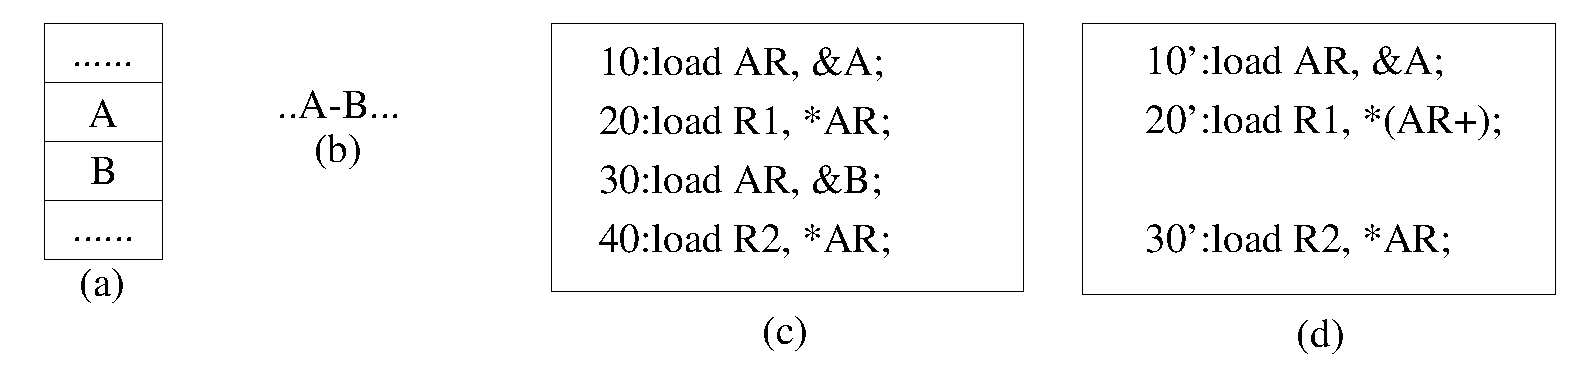
\includegraphics[scale=0.45]{figures/agu.eps}
	\label{fig:agu}
	\caption{Auto-addressing}
\end{figure}

The AGUs on DSP processors assist the address computation in parallel. For the most frequently used auto addressing instructions such as post- and pre- address increment/decrement instructions, no explicit addressing instruction is needed when the address distance of two consecutive memory accesses is smaller than two; otherwise an extra instruction is needed to update the address register (as instruction 30 shown in Figure~\ref{fig:agu}).

\textbf{Offset assignment}
Auto-addressing mode can increase the code performance as well as reducing code size. On the other hand, the memory layout has to be optimal in order to achieve the best code performance and compression. The problem of assigning variables in memory was formulated by Bartley~\cite{related:bartley} and Liao \textit{et al.}~\cite{related:liao} as Simple Offset Assignment (SOA) problem, where there is only one AR, and General Offset Assignment (GOA) problem, where there are multiple ARs. A variety of heuristic algorithms have been proposed later~\cite{related:atri,related:choi,related:leupers-1996,related:leupers-1998,related:ottoni,related:rao,related:sudarsanam,related:zhuang}.

The general solution of SOA is equivalent to finding the maximum weight Hamiltonian path\footnote{A Hamiltonian path in a graph is a path that visits every vertex exactly once.} in the access graph~\cite{related:bartley, related:liao}, where each vertex represents a variable; each edge between two vertices represents there is at least one consecutive access between the two related variables; and the weight of each edge shows the number of times that the two variables are consecutively accessed. GOA problem can be simplified as \textit{N} SOA problems, where \textit{N} is the AR number. 

\textbf{Offset Assignment with variable coalescing}
Since many variables have short live ranges, variables that do not interfere with each other can be allocated in the same memory location, to furthermore reduce data memory size and improve code performance. An efficient offset assignment heuristic using variable coalescing is proposed by Ottoni \textit{et al.}~\cite{related:ottoni} and Zhuang \textit{et al.} ~\cite{related:zhuang}. In each iteration, either an unselected edge is selected to be on the Hamiltonian path, or two vertices are chosen to be coalesced until no more vertices can be coalesced and the Hamiltonian path is built.

The design goal of the current offset assignment schemes is to generate efficient code with compact code size and improved performance. So when the program is slightly updated, the compiler might generate a different coalesced offset assignment compared to the original version. Even though the memory layout difference is very simple, e.g. when there is a simple switch of two variables' memory addresses, all the instructions that access these two variable or the instructions that are adjacent to the memory access instructions of these two variables may need to apply a different addressing mode, which produces many code differences from the original version. 
Thus, while doing software update in WSNs, we need the compiler to consider the memory layout similarity with the previous version of code, as well as the code efficiency and size, in order to reduce the patch size during software update.


\section{Patch generator}

After the code compilation is finished, the sink node generates the patch code based on the binary code before sending out the patches. There are several ways to prepare the patches.

\textbf{Compression}
Compression algorithms, such as bzip2, compress, LZO, PPMd and zlib, can be used on the generated binary code to reduce the patch size. Simply using these existing compression algorithms on the binary code generated by the compiler can reduce the patch size by 20\%~70\%. Even though it can help reduce the transmission power consumption, these high compression ratio algorithms also requires a lot of computation to retrieve the original code. Experiment results~\cite{related:barr-energy} show that bzip2 requires to run 31 instructions to restore 1 bit, which makes the code decompression very expensive.

\textbf{Differential patching}
When an update is an incremental improvement on a deployed function, such as bug fix or parameter change, the new image is often very similar as the old version. So instead of transmitting the complete image of the updated/new application, a differential patch between two images can be transmitted as the update. 
%An update script can be used to describe the differences~\cite{related:script, related:jeong-script, ucc}.
%After sensors receive the patch packets, they copy part of the code from the old image and part of the code from the patch, to form the updated binary.
However, this method only works well for small updates. When the update is relatively big, the patch size may be big.
%My study has shown that a simple source code level update can trigger big binary level differences, such as data allocation switching, register assignment switching and target address switching. For example, Reijers \textit{et al.} proposed a new script command called ``patch list'', which shifts the target address in the old image with an offset while copying the instruction to the new image.

Differential patching scheme can be used in our WSN software update framework design, because the update-conscious compilation technique could reduce the image differences. As discussed before, a small register assignment or data assignment change could cause a big difference in the generated target code, which may affect several instructions. The current differential patching schemes only show the instruction level differences in the script, which may need to incorporate multiple instruction changes in the update script. However, if the context-aware information, such as register assignment change or data assignment change is provided in the script, the sensors may be able to update the binary code by itself, which can significantly reduce the update patch size.

\textbf{High level instruction}
Patching code at higher semantic levels tends to generate smaller update script. Levis \textit{et al.} showed that the code size is very short when they are represented using virtual machine instructions~\cite{mate}. Marr\'on \textit{et al.} proposed a scheme to produce separate object files for TinyOS~\cite{tinyos} components and linked by sensors~\cite{related:flexcup}. Dunkels \textit{et al.} further proposed a dynamical linker for this systems~\cite{related:dynamic1}. Koshy \textit{et al.} proposed to relocated modules and generate the binary using a remote linker~\cite{related:dynamic2}.
A drawback of releasing code not in the binary format but the higher level language is that it requires extra runtime overhead, which might be not acceptable for tightly resource-constrainted embedded system.

\section{Distribution protocol}

After the patch generation stage, the patches are ready to be distributed over the network. Many code distribution protocols have~\cite{spin,trickle,melete,deluge,mnp} been proposed.

\textbf{SA-WSN code distribution protocol}
In SA-WSNs, all the sensors run the same application, so the distribution protocol design in SA-WSNs focuses on the efficient flooding scheme, which sends the patch packets to all the sensors in the network. The original efficient data flooding scheme in WSN, called SPIN~\cite{spin} uses a three-way handshaking protocol, shown in Figure~\ref{fig:spin}. Each sensor broadcasts the software information (ADV messages) as advertisements. The sensors that need to update its software send a request (REQ) message to the code owners. And then the code owners respond with the DATA messages.

\begin{figure}[htbp]
	\centering
		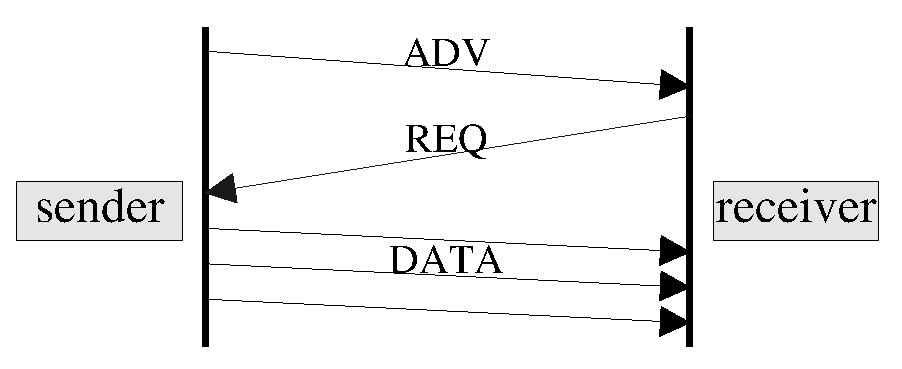
\includegraphics[scale=0.4]{figures/basic-protocol.eps}
	\label{fig:spin}
	\caption{Basic code distribution protocol (SPIN)}
\end{figure}

Trickle~\cite{trickle} improves SPIN by adding periodical advertisement feature, which reduces the energy used in the advertise phase. Deluge~\cite{deluge} extends Trickle to support efficient flooding of large data especially code images, by dividing big code image into fixed sized segments, and the transmission of different segments can happen simultaneously in the network for rapid code prorogation purpose. 


\textbf{MA-WSN code distribution protocol}
Because MA-WSNs support concurrent multiple application execution, only part of the sensors may be interested in the new code image. So a pull based multicast scheme should be used. Melete~\cite{melete} protocol only sends the code image to the sensors that request it instead of broadcasting it to all the sensors. Besides that, multihop code dissemination is also supported. The weakness of this scheme is that it relies on the request message to discover the routing to the source node, which may cause request message flooding in the network.


